\section{Unbelasteter Spannungsteiler} \label{c: Kapitel4}
Ein Spannungsteiler ist eine grundlegende Schaltung in der Elektrotechnik, die verwendet wird, um eine Eingangsspannung $U_{in}$ in eine proportionale Ausgangsspannung $U_{out}$ zu unterteilen. Dies wird durch die gezielte Auswahl und Dimensionierung zweier in Reihe geschalteter Widerstände $R_1$ und $R_2$ erreicht.

Die Ausgangsspannung wird dabei durch das Verhältnis der Widerstandswerte bestimmt und kann mit der folgenden Gleichung berechnet werden:
\begin{align} \label{eq:Spannungsteiler}
   U_{out} &= U_{in} \cdot \frac{R_2}{R_1 + R_2} = U_{in} \cdot k
\end{align}
In dieser Gleichung beschreibt der Faktor $k$ den Teilungsfaktor, der bestimmt, welcher Anteil der Eingangsspannung am Widerstand $R_2$ abfällt. Der Spannungsteiler ist ideal für Anwendungen, bei denen eine reduzierte Spannung benötigt wird, z. B. zur Anpassung eines Signals an einen bestimmten Eingangswert.

Ein wichtiger Aspekt eines unbelasteten Spannungsteilers ist, dass keine zusätzliche Last am Ausgang $U_{out}$ angeschlossen ist. Dadurch bleibt der Spannungsabfall ausschließlich durch die Widerstände $R_1$ und $R_2$ definiert. Sobald jedoch eine Last angeschlossen wird, verändert sich die Ausgangsspannung aufgrund des zusätzlichen Stroms, der durch die Last fließt.

Um diesen Zusammenhang besser zu verstehen, wird eine Schaltung gemäß Abbildung~\ref{fig:K4A1} aufgebaut. In dieser Schaltung werden die Spannungen $U_1$ und $U_2$ gemessen. Die gemessenen Werte werden anschließend in Tabelle \ref{tab:K4T1} dokumentiert und grafisch in Form von Kennlinien dargestellt (siehe Abbildung \ref{fig:K4A2}).
\vspace{0.5cm}
\begin{figure}[H]
    \centering
    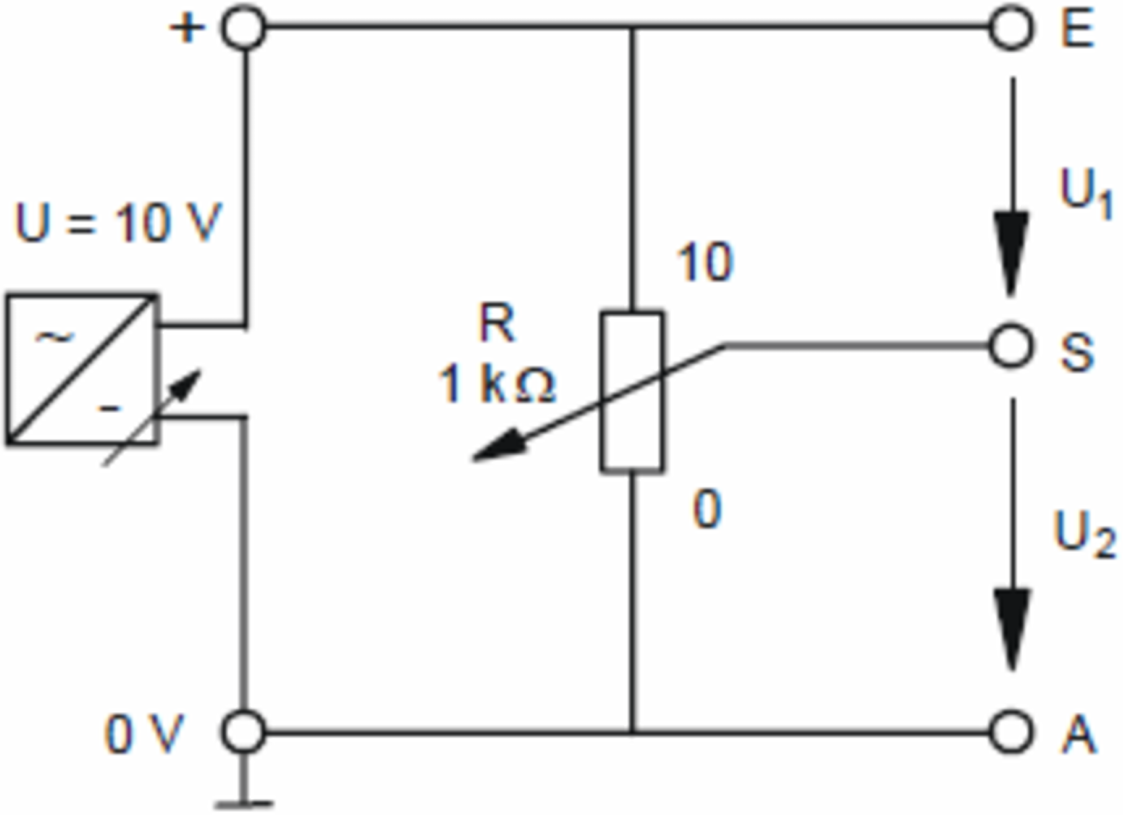
\includegraphics[width=0.5\textwidth]{Pictures/Kapitel4/Unbelasteter Spannungsteiler.png}
    \caption{Schematischer Aufbau unbelasteter Spannungsteiler}
    \label{fig:K4A1}
\end{figure}

\subsection{Messwerte}

Die Potentiometerstellung $\alpha$ gibt an, wie der Gesamtwiderstand $R$ auf die beiden Teilwiderstände $R_1$ und $R_2$ aufgeteilt wird. Ein hoher $\alpha$-Wert führt zu größeren Widerstanden von $R_2$ und kleineren von $R_1$, wodurch die Ausgangsspannung $U_2$ ansteigt.

\begin{table}[H]
\centering
\caption{Spannung $U$ bei Potentiometerstellung $\alpha$}
\begin{tabular}{ c c c c c c c c c c c c} % Abstand der Spalten
\toprule
    $\alpha$ & 0 & 1 & 2 & 3 & 4 & 5 & 6 & 7 & 8 & 9 & 10 \\
     \midrule
    $U_1/\,\unit{V}$ & 10,00 & 9,42 & 7,98 & 6,90 & 5,74 & 4,70 & 3,58 & 2,62 & 1,59 & 0,55 & 0,00 \\
    $U_2/\,\unit{V}$ & 0,00 & 0,58 & 2,02 & 3,09 & 4,24 & 5,28 & 6,39 & 7,35 & 8,38 & 9,42 & 10,00 \\
    \bottomrule
\end{tabular}
\label{tab:K4T1}%Rechnerische Tabelle2
\end{table}
\vspace{0.5cm}
\begin{figure}[H]
\centering
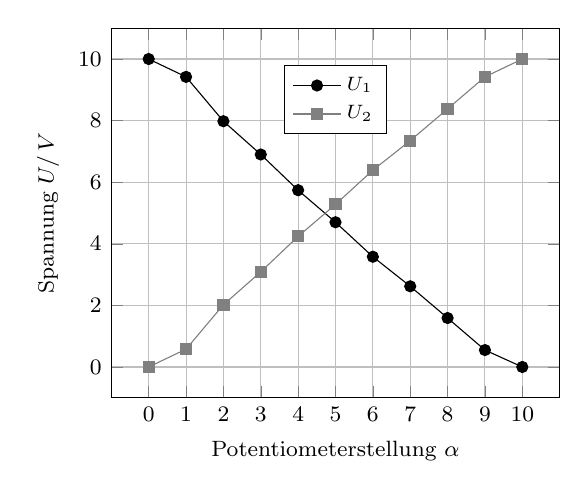
\begin{tikzpicture}
\begin{axis}[
    width=0.6\textwidth,
    xlabel={Potentiometerstellung $\alpha$},
    ylabel={Spannung $U/\,\unit{V}$},
    grid=major,
    legend style={at={(0.5,0.9)}, anchor=north, font=\scriptsize},
    xtick={0,1,2,3,4,5,6,7,8,9,10},
    xticklabels={0,1,2,3,4,5,6,7,8,9,10},
    ytick={0,2,4,6,8,10},
    font=\footnotesize
]

% Kennlinie U1
\addplot[mark=*,black] coordinates {
    (0,10.00) (1,9.42) (2,7.98) (3,6.90) (4,5.74) (5,4.70) (6,3.58) (7,2.62) (8,1.59) (9,0.55) (10,0.00)};
\addlegendentry{$U_1$}

% Kennlinie U2
\addplot[mark=square*,gray] coordinates {
    (0,0.00) (1,0.58) (2,2.02) (3,3.09) (4,4.24) (5,5.28) (6,6.39) (7,7.35) (8,8.38) (9,9.42) (10,10.00)};
\addlegendentry{$U_2$}

\end{axis}
\end{tikzpicture}
\caption{Kennlinie $U_1 =f(\alpha)$ und $U_2 =f(\alpha)$}
\label{fig:K4A2}
\end{figure}

Die berechneten Werte stimmen gut mit den gemessenen Spannungen überein. Abweichungen können auf Rundungsfehler oder geringe Messunsicherheiten zurückzuführen sein.

\newpage

\subsection{Rechnerische Überprüfung}

Die Messwerte aus Tabelle \ref{tab:K4T1} werden anhand der Gleichung~\eqref{eq:Spannungsteiler} überprüft. Die Ausgangsspannungen $U_1$ und $U_2$ hängen vom Verhältnis der Widerstände $R_1$ und $R_2$ ab. Für einen Gesamtwiderstand $R = 1\,\mathrm{k\Omega}$ und eine Eingangsspannung $U_{in} = 10\,\mathrm{V}$ gilt:

\[
U_1 = U_{in} \cdot \frac{R_1}{R_1 + R_2}, \quad U_2 = U_{in} \cdot \frac{R_2}{R_1 + R_2}
\]

Die Potentiometerstellung $\alpha$ bestimmt das Verhältnis von $R_1$ und $R_2$. Bei einer linearen Verteilung des Potentiometers gilt:

\begin{equation}
    R_1 = R \cdot \frac{\alpha}{10}
\end{equation}
\begin{equation}
    \quad R_2 = R \cdot \left( 1 - \frac{\alpha}{10} \right)
\end{equation}

Durch Einsetzen in die Spannungsteilerformel ergeben sich die berechneten Werte für $U_1$ und $U_2$, wie in Tabelle \ref{tab:K4T2} dargestellt:

\begin{table}[H]
\centering
\caption{Rechnerisch ermittelte Spannungen $U_1$ und $U_2$ bei Potentiometerstellung $\alpha$}
\begin{tabular}{c c c c c c c c c c c c}
\toprule
$\alpha$ & 0 & 1 & 2 & 3 & 4 & 5 & 6 & 7 & 8 & 9 & 10 \\
\midrule
$U_1/\,\unit{V}$ & 10,00 & 9,00 & 8,00 & 7,00 & 6,00 & 5,00 & 4,00 & 3,00 & 2,00 & 1,00 & 0,00 \\
$U_2/\,\unit{V}$ & 0,00 & 1,00 & 2,00 & 3,00 & 4,00 & 5,00 & 6,00 & 7,00 & 8,00 & 9,00 & 10,00 \\
\bottomrule
\end{tabular}
\label{tab:K4T2}
\end{table}

\newpage
